\documentclass{beamer}
%Information to be included in the title page:
\title[ANTIQUE Seminar]{ANTIQUE Seminar - Relational Symbolic Execution}
\author{Ignacio Tiraboschi}
\institute[INRIA / ENS]{INRIA Paris - ENS Paris}
\date{2022}
\usetheme{CambridgeUS}
\setbeamertemplate{page number in head/foot}[appendixframenumber]

% if then else in macros
\usepackage{xparse}
% inference rules
\usepackage{mathpartir}
% math fonts
\usepackage{amssymb}
\usepackage{amsthm}
\usepackage{amsmath}
\usepackage{stmaryrd}
\usepackage{mathtools}
\usepackage{mathrsfs}
\usepackage{latexsym}
%
\usepackage{tikz}
\usepackage{minted}
\usepackage{amsmath}
\usepackage{caption}
\usepackage{subcaption}
\usepackage[round,semicolon,authoryear,sort]{natbib}
\bibliographystyle{unsrtnat}
%
\RecustomVerbatimEnvironment{Verbatim}{BVerbatim}{}
\renewcommand{\figurename}{Listing}
%
\newcommand{\TODO}[1]{\noindent \textcolor{red}{\textsf{TODO: #1}}}
%
%%% Syntax %%%
\newcommand{\stnd}{\ensuremath{\textsf{stnd}}}
\newcommand{\implang}{\textsf{Imp}}
\NewDocumentCommand{\stmtskip}{ o }{
    \IfNoValueTF{#1}
        {\ensuremath{\textbf{skip}}}
        {\ensuremath{\textbf{skip}_#1}}
}
\NewDocumentCommand{\stmtassign}{ o m m }{
    \IfNoValueTF{#1}
        {\ensuremath{#2 := #3}}
        {\ensuremath{#2 \overset{#1}{:=} #3}}
}
\NewDocumentCommand{\stmtwhile}{ o o o }{
    % \IfNoValueTF{#1}
    %     {\textbf{while}}
    %     {\textbf{while} \; #1 \; \textbf{do} \; #2}
    \IfNoValueTF{#3}
        {\IfNoValueTF{#1}
            {\ensuremath{\mathbf{while}}}
            {\ensuremath{\mathbf{while} \; #1 \; \mathbf{do} \; #2}}
        }
        {\IfNoValueTF{#1}
            {\ensuremath{\mathbf{while}_#1}}
            {\ensuremath{\mathbf{while}_#3 \; #1 \; \mathbf{do} \; #2}}
        }
}
\NewDocumentCommand{\stmtloop}{ o o o }{
    % \IfNoValueTF{#1}
    %     {\textbf{loop}}
    %     {\textbf{loop} \; #1 \; \textbf{do} \; #2}
    \IfNoValueTF{#3}
        {\IfNoValueTF{#1}
            {\ensuremath{\mathbf{loop}}}
            {\ensuremath{\mathbf{loop} \; #1 \; \mathbf{do} \; #2}}
        }
        {\IfNoValueTF{#1}
            {\ensuremath{\mathbf{loop}_#1}}
            {\ensuremath{\mathbf{loop}_#3 \; #1 \; \mathbf{do} \; #2}}
        }
}
% \NewDocumentCommand{\stmtif}{ o o o }{
%     \IfNoValueTF{#1}
%         {\textbf{if}}
%         {\textbf{if} \; #1 \; \textbf{then} \; #2 \; \textbf{else} \; #3}
% }
\NewDocumentCommand{\stmtif}{ o o o o }{
    \IfNoValueTF{#4}
        {\IfNoValueTF{#1}
            {\ensuremath{\mathbf{if}}}
            {\ensuremath{\mathbf{if}\ #1\ \mathbf{then}\ #2\ \mathbf{else}\ #3}}
        }
        {\IfNoValueTF{#1}
            {\ensuremath{\mathbf{if}_#4}}
            {\ensuremath{\mathbf{if}_#4\ #1\ \mathbf{then}\ #2\ \mathbf{else}\ #3}}
        }
}
\NewDocumentCommand{\stmtseq}{ o o m }{
    \IfNoValueTF{#2}
        {\IfNoValueTF{#1}
            {\stmtskip ; #3}
            {#1 ; #3}
        }
        {\IfNoValueTF{#1}
            {\stmtskip \overset{#2}{;} #3}
            {#1 \overset{#2}{;} #3}
        }
}
\NewDocumentCommand{\wdepth}{ o }{
    \IfNoValueTF{#1}
        {\ensuremath{W_d}}
        {\ensuremath{W_d(#1)}}
}
\NewDocumentCommand{\comp}{ o o }{
    \IfNoValueTF{#1}
        {\ensuremath{\triangleright}}
        {\ensuremath{#1 \triangleright #2}}
}

%%% Semantics %%%
\newcommand{\eval}{\vdash}
\NewDocumentCommand{\sem}{ o }{
    \IfNoValueTF{#1}
        {\rightarrow}
        {\xrightarrow{#1}}
}
\NewDocumentCommand{\semW}{ o }{
    \IfNoValueTF{#1}
        {\rightarrow_\normW}
        {\xrightarrow{#1}_\normW}
}
\NewDocumentCommand{\semApp}{ o }{
    \IfNoValueTF{#1}
        {\rightarrow_\normApp}
        {\xrightarrow{#1}_\normApp}
}
\NewDocumentCommand{\semDApp}{ o }{
    \IfNoValueTF{#1}
        {\rightarrow_{\normD\normApp}}
        {\xrightarrow{#1}_{\normD\normApp}}
}
\NewDocumentCommand{\sse}{ o }{
    \IfNoValueTF{#1}
        {\rightharpoonup_s}
        {\xrightharpoonup{#1}_s}
}
\newcommand{\sseSet}{\overset{S}{\rightharpoonup}_s}
\NewDocumentCommand{\dse}{ o }{
    \IfNoValueTF{#1}
        {\rightharpoonup_d}
        {\xrightharpoonup{#1}_d}
}
\newcommand{\dseSet}{\overset{S}{\rightharpoonup}_d}
\newcommand{\apron}{\rightsquigarrow_\mathcal{A}}
\newcommand{\prSem}{\rightsquigarrow^{\mathcal{S}\times\mathcal{A}}}

%%% Notation %%%
\newcommand{\msingle}[1]{\langle #1 \rangle}
\newcommand{\mpair}[2]{\langle #1\ ; #2 \rangle}
\newcommand{\Mem}{\normalfont \textsf{Mem}}
\newcommand{\mem}{\mu}
\newcommand{\Stmt}{\ensuremath{\mathbf{Stmt}}}
\newcommand{\Expr}{\normalfont \mathbf{Expr}}
\newcommand{\Var}{\normalfont \textsf{Var}}
\newcommand{\Val}{\normalfont \textsf{Val}}
\newcommand{\SVal}{\normalfont \textsf{SVal}}
\newcommand{\Low}{\normalfont \textsf{Low}}
\newcommand{\High}{\normalfont \textsf{High}}
\newcommand{\true}{\textbf{tt}}
\newcommand{\false}{\textbf{ff}}
\newcommand{\Trc}{\normalfont \textsf{Trc}}
\newcommand{\lproj}{\textsf{left}}
\newcommand{\rproj}{\textsf{right}}
\newcommand{\prog}{\textsf{P}}

% Notation: non-interference
\newcommand{\loweq}{=_{\textsf{L}}}
\NewDocumentCommand{\niti}{ o }{
    \IfNoValueTF{#1}
        {\ensuremath{\mathcal{NI}^\mathit{T.I}}}
        {\ensuremath{\mathcal{NI}^\mathit{T.I}_#1}}
}
\NewDocumentCommand{\nits}{ o }{
    \IfNoValueTF{#1}
        {\ensuremath{\mathcal{NI}^\mathit{T.S}}}
        {\ensuremath{\mathcal{NI}^\mathit{T.S}_#1}}
}

% Notation: Non-standard
\newcommand{\normW}{\ensuremath{\text{\normalfont W}}}
\newcommand{\normApp}{\ensuremath{\text{\normalfont App}}}
\newcommand{\normD}{\ensuremath{\text{\normalfont D}}}
\newcommand{\normDM}{\ensuremath{\text{\normalfont DM}}}
\newcommand{\memW}{\ensuremath{\mem_\normW}}
\newcommand{\memApp}{\ensuremath{\xi}}
\newcommand{\memDApp}{\ensuremath{\xi_\normD}}
\newcommand{\MemW}{\ensuremath{\Mem_\normW}}
\newcommand{\MemApp}{\ensuremath{\Mem_\normApp}}
\newcommand{\MemDApp}{\ensuremath{\Mem_{\normD\normApp}}}
\newcommand{\stndW}{\ensuremath{\textsf{stnd}_\normW}}
\newcommand{\stndApp}{\ensuremath{\textsf{stnd}_\normApp}}
\newcommand{\relstdW}{\ensuremath{\equiv^\natural}}
\newcommand{\relWM}{\ensuremath{\in^\natural}}
\newcommand{\relAppSS}{\sat_\normApp}
\newcommand{\relDAppDS}{\sat_{\normD\normApp}}
% \newcommand{\eqdef}[1]{\overset{#1}{=\joinrel=}}
\newcommand{\eqlab}{\overset{\textbf{\footnotesize lab}}{=\joinrel=}}
% \newcommand{\eqlab}{\eqdef}
\newcommand{\neqlab}{\overset{\textbf{\footnotesize lab}}{=\joinrel\mathrel/\joinrel=}}
% \newcommand{\neqlab}{\not\eqlab}

% Notation: Dependences
\newcommand{\Dep}{\text{\normalfont Dep}}
\newcommand{\dep}{\ensuremath{\mathscr{D}}}
\newcommand{\depsem}{\Rrightarrow}
\newcommand{\depleq}{\sqsubseteq^\natural}
\newcommand{\deple}{\sqsubset^\natural}
\newcommand{\depsup}{\sqcup^\natural}
\newcommand{\depeval}[1]{\llparenthesis #1 \rrparenthesis^\natural}
\newcommand{\lagree}[3]{\mathcal{O}^#1 \depeval{#2} #3}
\newcommand{\alphahs}{\alpha_\text{hs}}

% Notation: Single-symbolic
\newcommand{\Sstate}{\mathbf{K}}
\newcommand{\SExpr}{\mathbf{SExpr}}
\NewDocumentCommand{\sat}{ o }{
    \IfNoValueTF{#1}
        {\vDash}
        {\vDash_{#1}}
}
\newcommand{\unsat}{\nvDash}
\newcommand{\relates}{\sat}
\newcommand{\smap}{\rho}
\newcommand{\spath}{\pi}
\newcommand{\lcount}{\text{\normalfont W}}
\newcommand{\sstate}{\kappa}
\newcommand{\seval}{\vdash_{\text{s}}}
\newcommand{\maxite}{\textsc{Max-ite}}
\newcommand{\wnew}{\textsf{w-new}}
\newcommand{\wincr}{\textsf{w-incr}}
\newcommand{\wdelete}{\textsf{w-delete}}
\newcommand{\wcounter}{\textsf{w-counter}}
\newcommand{\niter}[2]{\stackrel{\mathclap{\normalfont\mbox{#2}}}{#1}}

% Notation: Double-symbolic
\newcommand{\dstate}{\chi}
\newcommand{\Dstate}{\mathbf{X}}
\newcommand{\deval}{\vdash_{\text{d}}}
\newcommand{\init}{\normalfont\textsf{init}}
\newcommand{\eq}{\normalfont\textsf{eq}}
\newcommand{\analysis}{\normalfont\textsf{analysis}}

%%% Functions %%%
\newcommand{\modif}{\normalfont \textsf{modif}}
\newcommand{\fresh}{\normalfont \textsf{fresh}}
\newcommand{\filter}{\normalfont\textsf{filter}}
\newcommand{\new}{\normalfont \textsf{new}}
\newcommand{\lab}{\ensuremath{\mathbf{lab}}}

%%% Random %%%
\newcommand{\down}[1]{\rotatebox[origin=c]{270}{\ensuremath{#1}}}
\newcommand{\infersize}{\footnotesize}
\newcommand{\llcurly}{\{\joinrel\mathrel|}
\newcommand{\rrcurly}{\mathrel|\joinrel\}}
%
\begin{document}

\frame{\titlepage}

\begin{frame}
  \frametitle{Outline}
  \begin{enumerate}
    \item Symbolic execution.
    \begin{itemize}
      \item What is Symbolic execution?
      \item Example.
      \item Pros and cons.
    \end{itemize}
    \item Hyperproperties.
    \begin{itemize}
      \item Noninterference.
    \end{itemize}
    \item Symbolic execution for noninterference: \emph{Relational symbolic execution}.
    \begin{itemize}
      \item Example.
      \item How to achieve soundness?
    \end{itemize}
    \item 
  \end{enumerate}
\end{frame}

\begin{frame}
  \frametitle{Symbolic execution}
  \emph{Symbolic execution} executes the program over \textbf{symbolic variables and values} which
  \textbf{represent possible concrete values}.
  
  \pause
  \vspace{1em}
  Symbolic execution is very expressive and precise, and this is particularly good to find
  security vulnerabilities.
  
  \pause
  \vspace{1em}
  It is only \emph{sound up to a bound}. We can only unroll loops a limited amount of times.

  \pause
  \vspace{1em}
  It relies on an off-the-shelf SMT solver to handle satisfiabilty queries, which can eventually
  be a problem when queries are too complicated. Also, if not careful, there is
  \textbf{path explosion} \citep{DBLP:journals/cacm/CadarS13}.
\end{frame}

\begin{frame}
  \frametitle{Symbolic execution}
  More precisely, symbolic state is a pair $(\rho,\pi)$ where $\rho$ is the symbolic mapping and
  $\pi$ is the symbolic path.

  \vspace{1em}
  A regular safety property could be ``the program never divides by zero'' .
  To check this we need to see that:
  \begin{center}
    In all possible traces, no trace ever divides by zero.
  \end{center}

  \vspace{1em}
  Let us see an example to understand how we can use symbolic execution for verification.
\end{frame}

\begin{frame}[fragile]
  \frametitle{Example}
  \begin{figure}[htp]
    \centering
    \begin{minted}{c}
int x, y;
if (x != 0) {
  y = y / x;
}
    \end{minted}
  \end{figure}
  \begin{figure}
    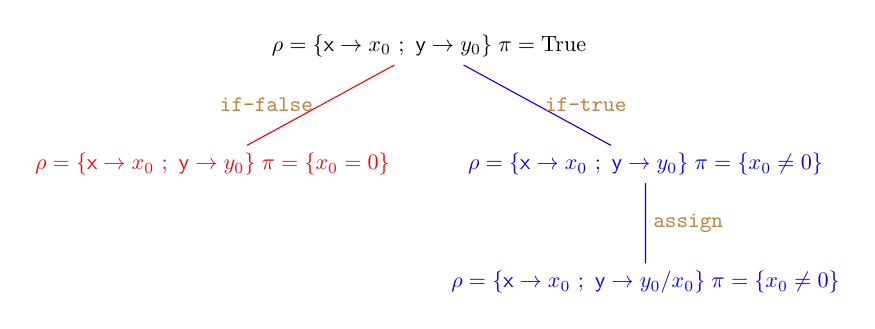
\begin{tikzpicture}
      \node[scale=0.8] { $\rho = \{ \textsf{x} \rightarrow x_0\ ;\ \textsf{y} \rightarrow y_0 \} \;
              \pi = \text{True}$ } [sibling distance = 5.5cm]
        child [red] {
          node [scale=0.8] {
            $\rho = \{ \textsf{x} \rightarrow x_0\ ;\ \textsf{y} \rightarrow y_0 \} \;
            \pi = \{ x_0 = 0 \}$
            } edge from parent node [scale=0.8, left, brown] {\texttt{if-false}}}
        child [blue] {
          node [scale=0.8] {
            $\rho = \{ \textsf{x} \rightarrow x_0\ ;\ \textsf{y} \rightarrow y_0 \} \;
            \pi = \{ x_0 \not = 0 \}$
            }
            child {node [scale=0.8] {
              $\rho = \{ \textsf{x} \rightarrow x_0\ ;\ \textsf{y} \rightarrow y_0 / x_0 \} \;
              \pi = \{ x_0 \not = 0 \}$
              } edge from parent node [scale=0.8, right, brown] {\texttt{assign}}}
            edge from parent node [scale=0.8, right, brown] {\texttt{if-true}}};
    \end{tikzpicture}
  \end{figure}
\end{frame}

\begin{frame}
  \frametitle{Symbolic execution}
  The previous example works great... \pause but what if we had loops?
  
  \vspace{1em}
  The usual method to deal with loops is to unfold up to certain bound, losing capability to actually
  verify a property.
  But this still allows finding vulnerabilities in the program.
\end{frame}

\begin{frame}
  \frametitle{Noninterference}
  The previous property depends only on individual traces.

  \vspace{1em}
  A \textbf{2-safety} \citep{Clarkson2008} property is a safety property over sets of traces.
  One 2-safety property of interest is \emph{noninterference}.

  \pause
  \vspace{1em}
  Noninterference is a confidentiality policy that stipulates commands executed on behalf of
  users holding \textbf{high clearances have no effect} on system behavior observed by users holding
  \textbf{low clearances}.

  \pause
  \begin{center}
    For any two traces initially agreeing on public values, if the traces end, they agree on its
    public values.
  \end{center}
\end{frame}

\begin{frame}
  \frametitle{Relational symbolic execution}
  In \emph{relational symbolic execution} \citep*{DBLP:journals/corr/abs-1711-08349} the authors
  propose a framework for verification of properties such as noninterference.
  
  \pause
  \vspace{1em}
  In relational symbolic execution we have that each variable is mapped to either one or two
  symbolic expressions.
  \[
    \textsf{x} \rightarrow \mpair{x_0}{x_1} \qquad \textsf{y} \rightarrow \msingle{y_0}
  \]

  \pause
  This allows for optimization:
  \begin{itemize}
    \item Low clearance variables cannot branch leading to fewer symbolic paths to follow.
    \item This also means that we execute fewer queries to the SMT solver.
  \end{itemize}
  \centering
  \textbf{Now we also have many possible combinations of paths!}
\end{frame}

\begin{frame}[fragile]
  \frametitle{Example}
  \begin{figure}[htp]
  \centering
  \begin{minted}{c}
if (x > 0) {
  y = 10;
}
  \end{minted}
  \end{figure}
  \begin{figure}
    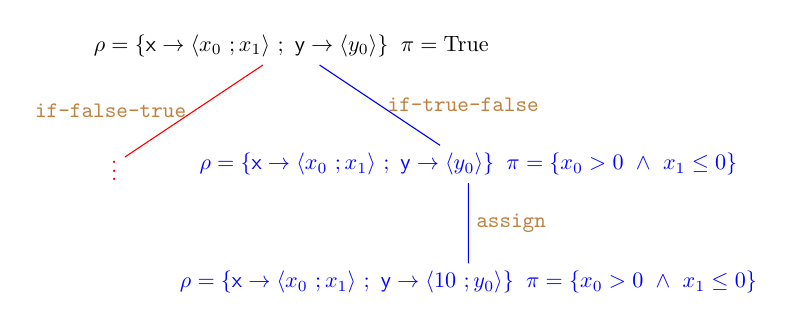
\begin{tikzpicture}
      \node[scale=0.8] { $\rho = \{ \textsf{x} \rightarrow \mpair{x_0}{x_1}\ ;\ \textsf{y} \rightarrow \msingle{y_0} \} \;\;
              \pi = \text{True}$ } [sibling distance = 4.5cm]
        child [red] {
          node [scale=0.8] { \vdots } edge from parent node [scale=0.8, left, brown] {\texttt{if-false-true}}}
        child [blue] {
          node [scale=0.8] {
            $\rho = \{ \textsf{x} \rightarrow \mpair{x_0}{x_1}\ ;\ \textsf{y} \rightarrow \msingle{y_0} \} \;\;
            \pi = \{ x_0 > 0\ \wedge\ x_1 \leq 0 \}$
            }
            child {node [scale=0.8] {
              $\rho = \{ \textsf{x} \rightarrow \mpair{x_0}{x_1}\ ;\ \textsf{y} \rightarrow \mpair{10}{y_0} \} \;\;
              \pi = \{ x_0 > 0\ \wedge\ x_1 \leq 0 \}$
              } edge from parent node [scale=0.8, right, brown] {\texttt{assign}}}
            edge from parent node [scale=0.8, right, brown] {\texttt{if-true-false}}};
    \end{tikzpicture}
  \end{figure}
\end{frame}

\begin{frame}
  \frametitle{Vulnerabilities in Relational symbolic execution}
  In the previous example, we are able to see that at least one relational trace is violating
  noninterference.

  \vspace{1em}
  Thanks to the SMT solver, we are able to get a model of showing the vulnerability. We can also
  reconstruct the path by looking at the symbolic path $\spath$.
\end{frame}

\begin{frame}
  \frametitle{Soundness in Relational symbolic execution}
  As we noted earlier, symbolic execution usually gives up on soundness and is used to find
  vulnerabilities.

  \vspace{1em}
  In the framework of Relational symbolic execution what is done is to \textbf{manually set invariants}
  to over approximate loops, and skip the symbolic execution of loops.
\end{frame}



\begin{frame}[allowframebreaks]
\frametitle{Bibliography}
\bibliography{main}
\end{frame}

\end{document}
